\chapter{Methodology}\label{chap:method}

\section*{}

In this chapter we intend to describe the methodology to be followed on this 
dissertation and propose a work plan.

% Este capítulo deve começar por fazer uma apresentação detalhada do
%problema a resolver\footnote{Na introdução a apresentação do
%  problema foi breve.} podendo mesmo, caso se justifique,
%constituir-se um capítulo com essa finalidade.
 
%Deve depois dedicar-se à apresentação da solução sem detalhes de
%implementação. 
%Dependendo do trabalho, pode ser uma descrição mais teórica, mais
%``arquitetural'', etc.

\section{Methodology} \label{sec:meth}

Like any software development project, a simulation project also has a life 
cycle. In this section we describe the steps to apply in the simulation 
methodology, based on Ulgen et al.~\cite{Ulgen1994} and Banks et 
al.~\cite[section 1.11]{Banks2004}, which can be summarized as follows:

\begin{enumerate}
    \item \textit{Problem formulation}: Clear statement of the problem by the 
    analyst and stakeholders; \label{enum:mform}
    \item \textit{Setting of objectives and overall project plan}: Questions to 
    be answered by the simulation, plans for the study, cost and number of days 
    for each phase, with the results expected at each stage; \label{enum:mobj}
    \item \textit{Model conceptualization}: Select, modify and iterate over the 
    assumptions that characterize the system; \label{enum:mconcept}
    \item \textit{Data collection}: Collect the necessary data to run and 
    validate the model, assuming that required data will change with the 
    increasing complexity of the system; \label{enum:mdata}
    \item \textit{Model translation}: Materialization of the system in a 
    program; \label{enum:mtransl}
    \item \textit{Verification}: Making sure that the program behaves correctly 
    accordingly to its inputs; \label{enum:mverif}
    \item \textit{Validation}: Calibration of the model, comparing the model 
    against an actual system; \label{enum:mvalid}
    \item \textit{Experimental design}: Tweak the experiments, comparing 
    alternative designs; \label{enum:mexp}
    \item \textit{Production runs and analysis}: Estimate measures of 
    performance for the systems that are being simulated; \label{enum:mprod}
    \item \textit{Documentation and reporting}: Document both the program and 
    the progress of the study; \label{enum:mdocs}
    \item \textit{Implementation}: End result of the study, including the 
    entire simulation process. \label{enum:mimpl}
\end{enumerate}

This process can be visualized in figure \ref{fig:sim}.

\begin{figure}[h]
    \begin{center}
        \leavevmode
        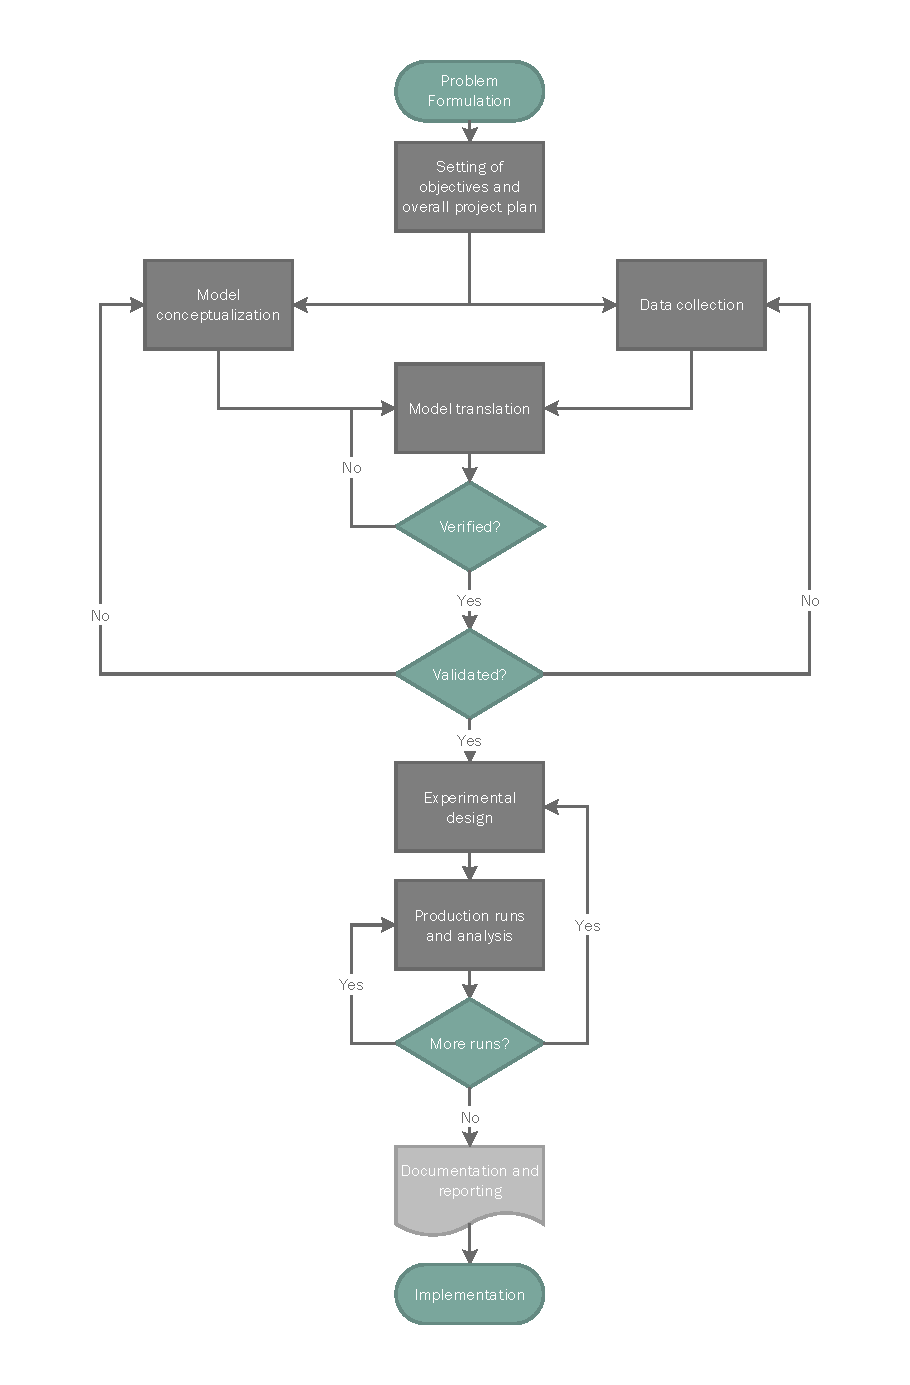
\includegraphics[width=0.6\textwidth]{simulation_study}
        \caption{Steps in a simulation study \cite{Banks2004}}
        \label{fig:sim}
    \end{center}
\end{figure}

\section{Planning}

Taking into account the steps described in section \ref{sec:meth}, a Gantt 
diagram was developed to define the tasks and their duration. This diagram is 
shown in appendix \ref{ap1:work_plan}.

We now present the details of the most important planned tasks. The name scheme 
follows \cite{Banks2004}.

\subsection{Discovery}

\begin{itemize}
    \item \textbf{Description}: Consists of the steps \textit{Problem 
    formulation} (\ref{enum:mform}) and \textit{Setting of objectives and 
    overall project plan} (\ref{enum:mobj}) presented above. In this stage the 
    initial statement of the problem and objectives are fine-tuned and 
    clarified.
    \item \textbf{Input}: Literature review on simulation, e-commerce and user 
    behaviour modelling and reunions with the supervisor.
    \item \textbf{Result}: Further clarification on the problem, overview and 
    analysis of the literature related with the dissertation and this report.
    \item \textbf{Time frame}: 01/10/2015 - 19/02/2016 (~20 weeks).
\end{itemize}

\subsection{Model building and data collection}

\begin{itemize}
    \item \textbf{Description}: Corresponds to the steps \ref{enum:mconcept} 
    to \ref{enum:mvalid} presented above. In this stage, the fundamental part 
    of the work is done and iterated multiple times. Emphasis should be given 
    to the reproducibility and validation of the process. This stage will be 
    further detailed during the dissertation period.
    \item \textbf{Input}: This report.
    \item \textbf{Result}: Runnable and testable simulation system, accompanied 
    by plausible scenarios (data) to feed the simulation.
    \item \textbf{Time frame}: 22/02/2016 - 15/04/2016 (~8 weeks).
\end{itemize}

\subsection{Running the model}

\begin{itemize}
    \item \textbf{Description}: Involves the steps \textit{Experimental design} 
    (\ref{enum:mexp}) and \textit{Production runs and analysis} 
    (\ref{enum:mprod}). In this stage, the model/system is tweaked and 
    statistical analysis is done on the experiment results.
    \item \textbf{Input}: Runnable simulation system.
    \item \textbf{Result}: Measurements of performance of the system being 
    evaluated.
    \item \textbf{Time frame}: 18/04/2016 - 06/05/2016 (~3 weeks).
\end{itemize}

\subsection{Implementation}

\begin{itemize}
    \item \textbf{Description}: Includes the steps \textit{Documentation and 
    reporting} (\ref{enum:mdocs}) and \textit{Implementation} 
    (\ref{enum:mimpl}). This final stage should conclude the dissertation, by 
    delivering the implementation of the framework/simulation engine and the 
    final dissertation report.
    \item \textbf{Input}: All the deliverables produced up to this point.
    \item \textbf{Result}: Documentation, dissertation report, concrete 
    simulation system implementation and verifiable results.
    \item \textbf{Time frame}: 09/05/2016 - 04/07/2016 (~8 weeks).
\end{itemize}

Architecture of the solution, implementation details (e.g. technologies) and on 
what actually consists a \textit{framework} were purposely left out of this 
planning dissertation report.
